\documentclass[border=10pt]{standalone}
\usepackage{amsmath}
\usepackage{tikz}
\usetikzlibrary{arrows.meta, fit, backgrounds, calc}

\definecolor{inputcol}{HTML}{4FC3F7}    % light blue
\definecolor{hiddencol}{HTML}{AB47BC}   % purple
\definecolor{outputcol}{HTML}{66BB6A}   % green — diagonal / target
\definecolor{attncol}{HTML}{FFA726}     % orange — special
\definecolor{skipcol}{HTML}{EF5350}     % red

\begin{document}
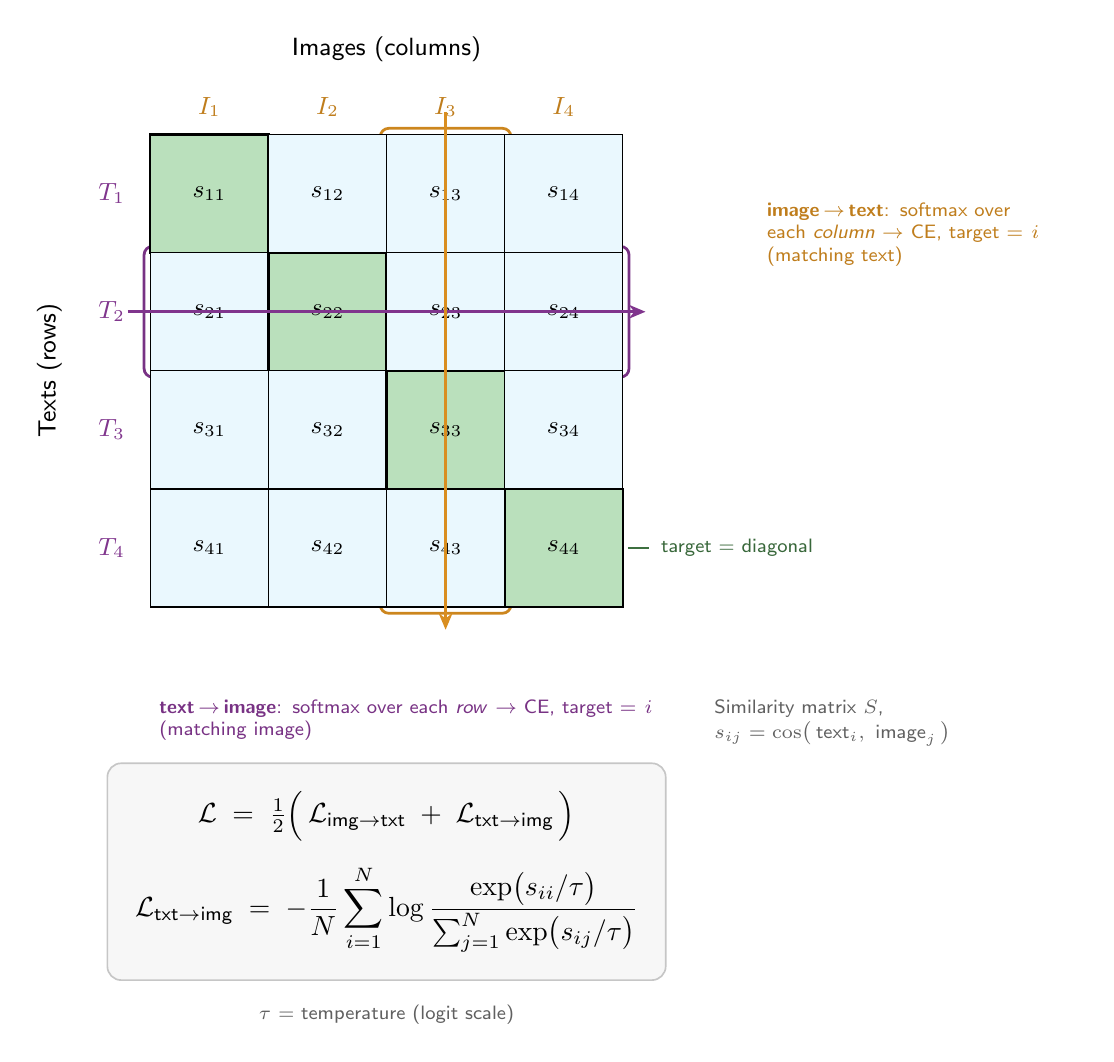
\begin{tikzpicture}[
    cellsize/.style={minimum width=1.5cm, minimum height=1.5cm},
    cell/.style={draw, cellsize, font=\sffamily\small, line width=0.5pt,
                 fill=inputcol!12},
    diag/.style={draw, cellsize, font=\sffamily\bfseries\small, line width=0.8pt,
                 fill=outputcol!45},
    axislabel/.style={font=\sffamily\small},
    annot/.style={font=\sffamily\scriptsize, text=gray!75!black},
    conn/.style={-{Stealth[length=6pt, width=5pt]}, line width=1pt}
  ]

  % ---- Grid geometry ----
  % columns x = 0..3 (images I_1..I_4), rows y = 0..-3 (texts T_1..T_4)
  \foreach \r in {0,1,2,3} {
    \foreach \c in {0,1,2,3} {
      \pgfmathtruncatemacro{\rr}{\r+1}
      \pgfmathtruncatemacro{\cc}{\c+1}
      \ifnum\r=\c
        \node[diag] (cell-\r-\c) at (1.5*\c, -1.5*\r)
          {$s_{\rr\rr}$};
      \else
        \node[cell] (cell-\r-\c) at (1.5*\c, -1.5*\r)
          {$s_{\rr\cc}$};
      \fi
    }
  }

  % ---- Column headers: images ----
  \foreach \c in {0,1,2,3} {
    \pgfmathtruncatemacro{\cc}{\c+1}
    \node[axislabel, attncol!75!black, anchor=south]
      at (1.5*\c, 0.85) {$I_{\cc}$};
  }
  \node[axislabel, anchor=south] at (2.25, 1.55) {Images (columns)};

  % ---- Row headers: texts ----
  \foreach \r in {0,1,2,3} {
    \pgfmathtruncatemacro{\rr}{\r+1}
    \node[axislabel, hiddencol!75!black, anchor=east]
      at (-0.95, -1.5*\r) {$T_{\rr}$};
  }
  \node[axislabel, rotate=90, anchor=south] at (-1.75, -2.25) {Texts (rows)};

  % ---- Diagonal "target" annotation ----
  \node[annot, text=outputcol!55!black, anchor=west]
    at ($(cell-3-3.east)+(0.35,0)$) {target = diagonal};
  \draw[outputcol!60!black, line width=0.8pt]
    ($(cell-3-3.east)+(0.05,0)$) -- ($(cell-3-3.east)+(0.32,0)$);

  % ============ text -> image : softmax over a ROW ============
  % highlight row r=1 (T_2)
  \begin{scope}[on background layer]
    \node[fit=(cell-1-0)(cell-1-3), draw=hiddencol!70!black, line width=1pt,
          rounded corners=3pt, inner sep=2pt] (rowbox) {};
  \end{scope}
  % directional arrow along the highlighted row, drawn just outside its left/right edges
  \draw[conn, hiddencol!75!black]
    ($(cell-1-0.west)+(-0.28,0)$) -- ($(cell-1-3.east)+(0.28,0)$);
  % annotation placed BELOW the grid, left side, so it never overlaps cells
  \node[annot, text=hiddencol!70!black, anchor=north west, align=left, text width=6.4cm]
    (rowannot)
    at ($(cell-3-0.south west)+(0,-1.05)$)
    {\textbf{text\,$\rightarrow$\,image}: softmax over each \emph{row} $\rightarrow$ CE, target $=i$ (matching image)};

  % ============ image -> text : softmax over a COLUMN ============
  % highlight column c=2 (I_3)
  \begin{scope}[on background layer]
    \node[fit=(cell-0-2)(cell-3-2), draw=attncol!80!black, line width=1pt,
          rounded corners=3pt, inner sep=2pt] (colbox) {};
  \end{scope}
  % directional arrow along the highlighted column, drawn just outside top/bottom edges
  \draw[conn, attncol!85!black]
    ($(cell-0-2.north)+(0,0.28)$) -- ($(cell-3-2.south)+(0,-0.28)$);
  % annotation placed to the RIGHT of the grid, clear of the column box
  \node[annot, text=attncol!75!black, anchor=north west, align=left, text width=3.6cm]
    at ($(cell-0-3.east)+(1.7,0)$)
    {\textbf{image\,$\rightarrow$\,text}: softmax over each \emph{column} $\rightarrow$ CE, target $=i$ (matching text)};

  % ---- Similarity-matrix caption (right of the row annotation, below grid) ----
  \node[annot, anchor=north west, align=left, text width=4.6cm]
    at ($(rowannot.north east)+(0.4,0)$)
    {Similarity matrix $S$,\\[1pt] $s_{ij}=\cos\!\big(\,\text{text}_i,\ \text{image}_j\,\big)$};

  % ---- Formula block underneath ----
  \node[draw=gray!45, rounded corners=5pt, fill=gray!6, line width=0.6pt,
        inner sep=10pt, font=\sffamily, align=center]
        (formula)
        at ($(cell-3-0.south)!0.5!(cell-3-3.south)+(0,-3.35)$)
    {$\displaystyle
       \mathcal{L} \;=\; \tfrac{1}{2}\Big(\,
       \mathcal{L}_{\text{img}\rightarrow\text{txt}}
       \;+\;
       \mathcal{L}_{\text{txt}\rightarrow\text{img}}\,\Big)$
     \\[8pt]
     $\displaystyle
       \mathcal{L}_{\text{txt}\rightarrow\text{img}}
       \;=\;
       -\frac{1}{N}\sum_{i=1}^{N}
       \log\frac{\exp\!\big(s_{ii}/\tau\big)}
                {\sum_{j=1}^{N}\exp\!\big(s_{ij}/\tau\big)}$};

  \node[annot, anchor=north]
    at ($(formula.south)+(0,-0.18)$)
    {$\tau$ = temperature (logit scale)};

\end{tikzpicture}
\end{document}
